\question (青岛大学,2000年)对关键字序列28,16,32,12,60,2,5,72快速排序,从小到大的一次划分结果为(
)
\par\fourch{(2,5,12,16)26(60,32,72)}{\textcolor{red}{(5,16,2,12)28(60,32,72)}}{(2,16,12,5)28(60,32,72)}{(5,16,2,12)28(32,60,72)}
\begin{solution}根据快速排序的执行过程,保存好第一个元素值28(``挖坑'')后,从右边开始找到第一个比该元素值小的数,然后填入第一个位置(``填坑''),即为5,排除A和C。然后新的``坑''即为原来5的位置,从左边开始找到第一个比元素值28大的数,即为32,填入倒数第二个位置,因此排除D。因此本题选B。
\end{solution}
\question (电子科技大学,2007年)对下列4个序列,以第一个关键字为基础用快速排序算法进行排序,在第一趟过程中移动记录次数最多的是(
)
\par\fourch{\textcolor{red}{92,96,100,110,42,35,30,88}}{92,96,88,42,30,35,110,100}{100,96,92,35,30,110,88,42}{42,30,35,92,100,96,88,110}
\begin{solution}A选项比92小的数都在最后,比92大的数都在前面,第一趟的结果是需要把后面的这些数都前移,前面的这些数都后移,因此需要最多的移动记录次数,即每次比较后都要进行移动。
\end{solution}
\question (华南理工大学,2007年)快速排序方法在( )情况下最不利于发挥其长处
\par\twoch{要排序的数据量太大}{要排序的数据中含有多个相同值}{要排序的数据个数为奇数}{\textcolor{red}{要排序的数据已基本有序}}
\begin{solution}快速排序最好情况下时间复杂度为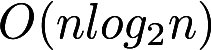
\includegraphics[width=0.76042in,height=0.18750in]{texmath/3043595Cdpi7B3507DO28nlog_2n29},待排序列越接近无序,本算法效率越高。最坏情况下时间复杂度为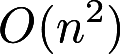
\includegraphics[width=0.43750in,height=0.19792in]{texmath/ead2f65Cdpi7B3507DO28n5E229},待排序列越接近有序,本算法效率越低,平均时间复杂度为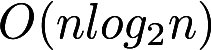
\includegraphics[width=0.76042in,height=0.18750in]{texmath/3043595Cdpi7B3507DO28nlog_2n29}。
\end{solution}
\question (武汉大学,2004年)对8个元素的线性表进行快速排序,在最好的情况下,元素间的比较次数为(
)
\par\twoch{7次}{8次}{12次}{\textcolor{red}{13次}}
\begin{solution}对8个元素排序的最好情况是:第一次找到的元素将原表分成长度为3和4的表,用7次比较;第二层,对于长度为3的表,最少需要2次,对于长度为4的表,继续分成长度为1和长度为2的表,最少需要3次;第三层,需要对长度为2的表进行排序,最少需要1次比较,所以总共需要7+2+3+1=13次。
\end{solution}
\question (中山大学,2004年)下列序列中,( )是执行第一趟快速排序后的结果
\par\fourch{\textcolor{red}{[30,50,36,10,81],85,[92,95]}}{[30,50,36,10],85,[92,81,95]}{[10,92,81,95],85,[30,50,36]}{[50,92,81,95],85,[10,30,36]}
\begin{solution}快速排序一趟后,枢轴左边的数据均小于枢轴,右边的数据均大于枢轴。
\end{solution}
\question (华中科技大学,2007年)下列排序方法中,(
)在待排序的数据为有序时,花费时间反而最多
\par\twoch{\textcolor{red}{快速排序}}{插入排序}{堆排序}{冒泡排序}
\begin{solution}快速排序最好情况下的时间复杂度为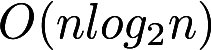
\includegraphics[width=0.76042in,height=0.18750in]{texmath/3043595Cdpi7B3507DO28nlog_2n29},待排序列越接近无序,本算法效率越高;最坏情况下的时间复杂度为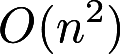
\includegraphics[width=0.43750in,height=0.19792in]{texmath/ead2f65Cdpi7B3507DO28n5E229},待排序列越接近有序,本算法效率越低。平均时间复杂度为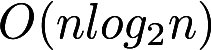
\includegraphics[width=0.76042in,height=0.18750in]{texmath/3043595Cdpi7B3507DO28nlog_2n29}。
\end{solution}
\question (厦门大学,2004年)对以下关键字序列用快速排序进行排序,( )速度最慢
\par\fourch{(19,23,3,15,7,21,28)}{(23,21,28,15,19,3,7)}{(19,7,15,28,23,21,3)}{\textcolor{red}{(3,7,15,19,21,23,28)}}
\begin{solution}快速排序的最坏情况为待排序表是有序的时候,由于D为有序表,所以本题选D。
\end{solution}
\question 采用递归方式对顺序表进行快速排序。下列关于递归次数的叙述中,正确的是(
)
\par\fourch{递归次数与初始数据的排列次数无关}{每次划分后,先处理较长的分区可以减少递归次数}{每次划分后,先处理较短的分区可以减少递归次数}{\textcolor{red}{递归次数与每次划分后得到的分区的处理顺序无关}}
\begin{solution}本题实际考察了快速排序的时间复杂度分析,快速排序的效率与初始序列有关这是显然的,因此A错。
对于B,C,D: 折半查找法的算法可以简写为: void qicksort(int R{[}{]},int
l,int r) \{ \ldots{} \ldots{} \ldots{} \ldots{} qicksort(R,l,i-1); //①
qicksort(R,i+1,r); //② \}
快速排序的递归次数由l和r决定(l和r决定了要处理问题的规模)。将快速排序的递归次数设为F(l,r),则按照上述代码中①②句的执行次序有:
递归次数F(l,r)=F(l,i-1)+F(i+1,r)\ldots{}\ldots{}\ldots{}.③
如果将①②句颠倒,则有:
递归次数F(l,r)=F(i+1,r)+F(l,i-1)\ldots{}\ldots{}\ldots{}.④
显然③和④式是相等的,因此递归次数与每次划分后得到的分区处理顺序无关。
【总结】
快速排序的基本思想是:通过一趟排序将要排序的数据分割成独立的两部分,其中一部分的所有数据都比另外一部分的所有数据小,然后再按此方法对这两部分数据分别进行快速排序,整个排序过程可以递归进行,以此达到整个数据变成有序序列。
\end{solution}
\question 下列选项中,不可能是快速排序第2趟排序结果的是( )
\par\twoch{2,3,5,4,6,7,9}{2,7,5,6,4,3,9}{\textcolor{red}{3,2,5,4,7,6,9}}{4,2,3,5,7,6,9}
\begin{solution}首先我们先学会判断一趟快速排序结果的特点,即以一个``枢轴'',将序列分成两部分,枢轴的一边全是比它小,另一边全是比它大。我们先来判断第1趟排序的``枢轴''。
对于A选项,第1趟的``枢轴''可能是2,6,7,9。考虑6的情况,将序列分为2,3,5,4和7,9。再用同样的方法判断这两段序列,都可能是一趟快速排序的结果,因此A可能是快速排序第2趟排序的结果。
对于B选项,第1趟的``枢轴''可能是2,9。考虑9的情况,将序列分为空序列和7,5,6,4,3,9。该序列也可能是以9为``枢轴''的一趟快排的结果,因此B也是可能选项。
对于C选项,第1趟的``枢轴''可能是9。考虑9的情况,将序列分为3,2,5,4,7,6和空序列。其中序列3,2,5,4,7,6找不到一个可能的``枢轴'',因此C不是可能选项。
最后D选项,第1趟的``枢轴''可能是5和9。考虑9的情况,将序列分为4,2,3,5,7,6和空序列,其中序列4,2,3,5,7,6的``枢轴'',可能是5,因此D也是可能选项。
\end{solution}
\question (北京师范大学,2004年)用某种排序方法对线性表\{24,88,21,48,15,27,69,35,20\}进行排序时,元素序列的变化情况如下:
(1)24,88,21,48,15,27,69,35,20 (2)20,15,21,24,48,27,69,35,88
(3)15,20,21,24,35,27,48,69,88 (4)15,20,21,24,27,35,48,69,88
则所采用的排序方法是( )
\par\twoch{\textcolor{red}{快速排序}}{选择排序}{希尔排序}{归并排序}
\begin{solution}如果是选择排序,则在4轮排序过程中无法得到最后的排序结构。如果是希尔排序不可能在第一步将20换到第一位。同理也不是归并排序。这4次过程中是子序列同时进行的快速排序
\end{solution}
